\documentclass[a4paper,12pt]{memoir}
\usepackage{msiu_term_work}

\lstset{language=Ruby,inputencoding=utf8/koi8-r,basicstyle=\small,
stringstyle=\ttfamily,xleftmargin=1cm}

\begin{document}
\renewcommand{\contentsname}{{\Large{Содержание}\hfill}}

\title{Методы хранения и обработки информации}
{Вычисление количества вершин выпуклой оболочки, лежащих в 1-окрестности
 заданного заполненного треугольника.
 Нахождение суммы длин проекций невидимых частей частично видимых рёбер,
  образующих с горизонтальной плоскостью угол не более $\pi/7$, центр 
  которых находится строго внутри сферы $x^2+y^2+z^2<4$}
{2362}
{Б.\+М.~Бирюков}
{к.ф.-м.н., доцент}
{Е.\+А.~Роганов}
{2014}

\section{Введение}
Проект «Выпуклая оболочка»\cite{convex} решает задачу индуктивного 
перевычисления 
выпуклой оболочки последовательно поступающих точек плоскости и таких её
характеристик, как периметр и площади выпуклой оболочки. Решение этой задачи требует знания теории индуктивных
функций~\cite{roganov-2002}, основ аналитической геометрии, векторной алгебры
и языка Ruby~\cite{ruby}.

Прoект «Изображение проекции полиэдра»~\cite{polyedr}~--- пример
классической задачи, для успешного решения которой необходимо знакомство с
основами вычислительной геометрии. Для этого необходимы хорошее понимание ряда разделов 
аналитической геометрии и векторной алгебры, основ объектно-ориентированного
программирования и языка Ruby. 

В данной курсовой работе рассматриваются модификации двух эталонных про-
ектов «Выпуклая оболочка» и «Изображение проекции полиэдра».
Целями работы являются:
\begin{enumerate}[1)]
\item в проекте «Выпуклая оболочка» вычислить количество пар вершин выпуклой оболочки, расстояние между которыми не превосходит единицу; 
\item в проекте «Изображение проекции полиэдра»  вычислить
сумму длин рёбер, середина и ровно один из концов которых находятся
на расстоянии строго меньше 1 от плоскости $\mathit x = 2$.

\end{enumerate}
Общее количество строк в рассмотренных проектах составляет около $000000000000$, из кoтoрых
бoлее $0000000000$ были изменены или дoбавлены автoрoм в прoцессе рабoты
над задачами мoдификации.
\section{Модификация проекта «Выпуклая оболочка»}

\subsection{Постановка задачи}

Модифицируйте эталонный проект таким образом, чтобы вычислялось количество пар вершин выпуклой оболочки, расстояние между которыми не превосходит единицу.
На начальном этапе работы программа запрашивает координаты вершин выпуклой оболочки, которая впоследствии индуктивно добавляет ее в выпуклую оболочку. Для решения нашей задачи необходимо выводить, помимо значений периметра и площади, количество пар вершин выпуклой оболочки, расстояние между которыми не превосходит единицу.

Для выполнения задания необходимо обладать базовыми знаниями в линейной алгебре. 2 точки, при их соединении, образуют отрезок, который можно представить в виде вектора. Чтобы получить длину (модуль) вектора $\overrightarrow{AB}$ необходимо воспользоваться следующей формулой:
$$\mid \overrightarrow{AB} \mid = \sqrt{(B_{x}-A_{x})^2+(B_{y}-A_{y})^2}$$  

Рассмотрим пример. Для последовательности точек $A(0, 0)$, $B(1, 0)$ и $C(0, 5)$ программа
выводит 1 в качестве количествa пар, расстояние между которыми не превосходит единицу.
После того,как мы вели  следующую точку $D(1, 5)$, количество ребер, расстояние между которыми не превосходит единицу, равняется $2$ (рис.~1).

\begin{figure}[ht!]
\begin{center}
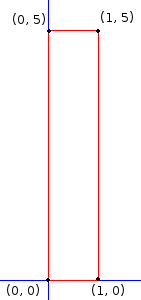
\includegraphics[scale=0.7]{images/picture1}
\center{\texttt{Рис.~1.}}
\end{center}
\end{figure}
\newpage

\sloppy Все требуемые функции будут вписываться в файлы проекта \texttt{convex.rb} и \texttt{r2point.rb}.

\subsection{Решение}

Для выполнения задания необходимо вычислять растояние между вершинами выпуклой оболочки. В эталонном проекте изначально присутствует функция \texttt{dist}, которая считает расстояние между вершинами выпуклой оболочки.
\subsection{Модификация кода}
При реализации кода были произведены изменения в четырех файлах эталонного проекта: \texttt{r2point.rb}, \texttt{convex.rb}, \texttt{run\_convex.rb}, \texttt{run\_tkconvex.rb}.
Рассмотрим  изменения кода в файле \texttt{r2point.rb}. В него был добавлен метод \texttt{distance}:

\begin{small}
\begin{verbatim}
class R2Point
...
  def distance(a)
    return (self.dist(a)<=1)? 1 : 0
  end
  ...
\end{verbatim}
\end{small}

Данный метод рассматривает две точки, и проверяет, не превышает ли расстояние между вершинами $1$. Для этого используется метод \texttt{dist} класса \texttt{R2Point}  В случае, если расстояние меньше либо равно единице, то метод \texttt{distance} возвращает значение 1, в противном случае, возвращается 0. На этом модификация файла \texttt{r2point.rb} завершена.
\newpage
Рассмотрим модификацию файла \texttt{convex.rb}. В классе \texttt{Segment} добавляется метод \texttt{dist}:

\begin{small}
\begin{verbatim}
class Segment < Figure
  ...
  def dist
    return (@p.dist(@q) <= 1)? 1 : 0
  end
  ...
\end{verbatim}
\end{small}

Этот метод проверяет длину двуугольника (отрезка). Если она больше единицы возвращается значение 0, иначе возвращается значение 1.

Затем редактируется класс \texttt{Polygon}. Первоначально при создании объекта класса \texttt{Polygon} создается треугольник. Необходимо при инициализации объекта посчитать расстояния между вершинами треугольника и узнать, сколько пар вершин, между которыми расстояние не более единицы.

\begin{small}
\begin{verbatim}
class Polygon < Figure
  attr_reader :points, :perimeter, :area

  def initialize(a, b, c)
    ...
    @dist = a.distance(b) + b.distance(c) + c.distance(a)
  end
  ...
\end{verbatim}
\end{small}

В последстви, при добавлении новых точек индуктивно вычисляется расстояние от добавляемой точки, до первой и последней вершин выпуклой облочки :

\begin{small}
\begin{verbatim}
  ...
  @perimeter += t.dist(@points.first) + t.dist(@points.last)
  @dist += t.distance(@points.first) + t.distance(@points.last)
  @points.push_first(t)
  ...
\end{verbatim}
\end{small}

Как и при добавлени, так и при удалении вычисляется расстояние между вершинами, и если расстояние между парами вершин превышает $1$, то удаляются из переменной.

\begin{small}
\begin{verbatim}
 p = @points.pop_first
   while t.light?(p, @points.first)
     @perimeter -= p.dist(@points.first)
     @area      += R2Point.area(t, p, @points.first).abs
     @dist      -= p.distance(@points.first)
     p  = @points.pop_first
   end
 @points.push_first(p)
  ...
  p = @points.pop_last
    while t.light?(@points.last, p)
      @perimeter -= p.dist(@points.last)
      @area      += R2Point.area(t, p, @points.last).abs
      @dist      -= p.distance(@points.last)
      p = @points.pop_last
    end
  @points.push_last(p)
\end{verbatim}
\end{small}

Далее расмотрим примеры работы программы. 
В случае, когда создается объект класса \texttt{Void} количество вершин выпуклой оболочки равно нулю. Когда добавляется вершина создается объект класса \texttt{Point}. В обоих случаях количество вершин оболочки меньше двух, считать расстояние между вершинами невозможно и возвращается число 0. При создании объектов классов \texttt{Segment} и \texttt{Polygon} количество вершин больше либо равно двум и необходимо считать расстояния между вершинами.
Для точек  с координатами$(0, 0)$ и $(1, 0)$ расстояние между которыми равно 1, следовательно, программа выведет 1 (рис.~2).

\begin{figure}[ht!]
\begin{center}
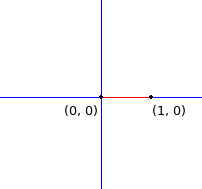
\includegraphics[scale=1.0]{images/picture2.png}
\center{\texttt{Рис.~2.}}
\end{center}
\end{figure}
\newpage
При добавелнии новой точки $(0, 1)$, расстояние между всеми точками пересчитывается, и программа выводит результат 2. Так как растояние между вершинами $(0, 0)$ и $(0, 1)$, $(0, 0)$ и $(1, 0)$ равно 1, а расстояние между вершинами $(0, 1)$ и $(1, 0)$ превосходит 1 (рис.~3).

\begin{figure}[ht!]
\begin{center}
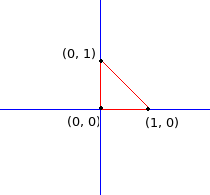
\includegraphics[scale=1.0]{images/picture3.png}
\center{\texttt{Рис.~3.}}
\end{center}
\end{figure}


При добавлении точки $(1, 1)$, программа пересчитывает расстояния между точками и выводит ответ $4$ (рис.~4).

\begin{figure}[ht!]
\begin{center}
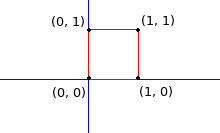
\includegraphics[scale=1.0]{images/picture4.png}
\center{\texttt{Рис.~4.}}
\end{center}
\end{figure}

\newpage
Далее добавляется новая точка $(1, 3)$. Точка $(1, 1)$ удаляется и выводится ответ 2 (рис.~5).

\begin{figure}[ht!]
\begin{center}
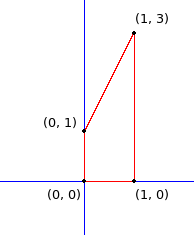
\includegraphics[scale=1.0]{images/picture5.png}
\center{\texttt{Рис.~5.}}
\end{center}
\end{figure}


\section{Модификация проекта <<Изображение проекции полиэдра>>}

\subsection{Постановка задачи}

Модифицируйте эталонный проект таким образом, чтобы определялась и печаталась следующая характеристика полиэдра: сумма длин рёбер, середина и ровно один из концов которых находится на расстоянии строго меньше $1$ от плоскости $x=2$. 
Для выполнения задания необходимо анализировать расположение середины и вершин всех ребер полиэдра относительно плоскости $x=2$. Для этого модифицируем эталонный проект, добавив необходимые методы нахождения середины ребра, расстояния от точки до плоскости $x=2$ и вычисления длины ребра.

\subsection{Решение задачи и модификация кода}
Чтобы определить, явялется ли точка хорошей, необходимо узнать находится ли координата $\mathit x$ любой точки на расстоянии строго меньше единицы от прямой $x=2$. Так как длина ~--- величина положительная будем использовать метод \texttt{abs}, позволяющий получить модуль числа, к которому применяется этот метод. Для определения, является ли точка удовлетворяющей условию, в классе \texttt{R3} файла \texttt{common/polyedr.rb}, добавим метод \texttt{good?}: 

\begin{small}
\begin{verbatim}
class R3
  ...
  def good?
    if (2.0 - @x).abs < 1.0 
      return true
    else
      return false
    end 
  end
  ...
\end{verbatim}
\end{small}

Ребро в нашем проекте является отрезком в пространстве, поэтому для нахождения середины ребра необходимо найти середину отрезка. Координаты середины отрезка в пространстве $[ \mathit a, \mathit b ]$ вычисляются по формуле:
$$x_{c}=\frac{a_{x}+b_{x}}{2};~y_{c}=~\frac{a_{y}+b_{y}}{2};~z_{c}=~ \frac{a_{z}+b_{z}}{2}.$$
В классе \texttt{Edge}, добавим метод, \texttt{center} который создает новую точку координаты которой находятся по формулам, указанным выше:

\begin{small}
\begin{verbatim}
class Edge
  ...
  def center
    xc=(@fin.x+@beg.x)/2.0 
    yc=(@fin.y+@beg.y)/2.0
    zc=(@fin.z+@beg.z)/2.0
    return R3.new(xc,yc,zc)
  end
  ...
\end{verbatim}
\end{small}


Так же добавим метод \texttt{length}, который возвращает длину ребра, где переменная \texttt{coef} явлется коэффициентом гомотетии.

\begin{small}
\begin{verbatim}
class Edge
  ...
  def length 
     Math.sqrt(((@fin.x-@beg.x)**2+(@fin.y-@beg.y)**2+(@fin.z-@beg.z)**2))/@coef
  end
  ...
\end{verbatim}
\end{small}

Далее добавим метод \texttt{func} в классе \texttt{Polyedr} возвращающий сумму длин рёбер, середина и ровно один из концов которых — «хорошие» точки.

\begin{small}
\begin{verbatim}
class Polyedr
  ...
  def func 
    sum=0
    edges.each do |e|
      if e.center.good?(e.coef) && (e.beg.good?(e.coef) ^ e.fin.good?(e.coef))
        sum += e.length
      end
    end
    return sum
  end
  ...
\end{verbatim}
\end{small}

После этого остается модифицировать файл, запускающий программу.

\begin{small}
\begin{verbatim}
#!/usr/bin/env ruby
# encoding: UTF-8
require './polyedr'
require '../common/tk_drawer'
TkDrawer.create
%w(test1 ).each do |name|
  puts '============================================================='
  puts "Начало работы с полиэдром '#{name}'"
  start_time = Time.now
  a=Polyedr.new("../data/#{name}.geom")
  a.draw 
  puts a.func
  puts "Изображение полиэдра '#{name}' заняло #{Time.now - start_time} сек."
  print 'Hit "Return" to continue -> '
  gets
end

\end{verbatim}
\end{small}

Модификация завершена. Работа программы с тестовым файлом \texttt{test1.geom} (рис.~6):

\begin{figure}[ht!]
\begin{center}
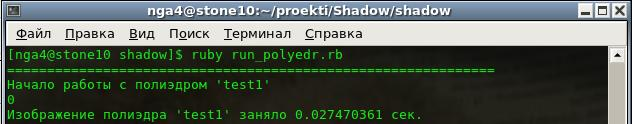
\includegraphics[scale=0.7]{images/6.jpg}
\center{\texttt{Рис.~6.}}
\end{center}
\end{figure}

Сам файл:

\begin{small}
\begin{verbatim}
10.0	0.0	0.0	0.0
4	1	4
1.5 0.0 0.0
3.5 0.0 0.0
3.5 5.0 0.0
1.5 5.0 0.0
4	1    2    3    4    
\end{verbatim}
\end{small}








\begin{thebibliography}{}

\bibitem{convex}
\link{http://edu.msiu.ru//files/25029-lecture.html}~---
Описание проекта «Выпуклая оболочка».

\bibitem{roganov-2002}
Е.А. Роганов
{\em Основы информатики и программирования.}~---
М., МГИУ, 2002.

\bibitem{ruby}
\link{http://ru.wikipedia.org/wiki/Ruby}~---
Википедия (свободная энциклопедия) о языке Ruby.

\bibitem{polyedr}
\link{http://edu.msiu.ru/files/26490-lecture.html}, 

\link{http://edu.msiu.ru/files/26929-lecture.html}~---
Описание проекта «Изображение проекции полиэдра».

\bibitem{latex}
\link{http://www-sbras.nsc.ru/win/docs/TeX/LaTex2e/Text\_in\_LaTeX.pdf}~---
Справочник по командам LATEX.

\bibitem{proizv}
\link{http://ru.wikipedia.org/wiki/Скалярное\_произведение}~---
Статья о скалярном произведении

\bibitem{dist}
\link{http://ru.onlinemschool.com/math/library/analytic\_geometry/p\_plane/}~---
Расстояние от точки до плоскости
\end{thebibliography}


\end{document}
